\label{section:1d_column_example}
This example \footnote{See verification example   \texttt{MUT\_Examples$\backslash$1\_VSF\_Column}} simulates variably-saturated flow in a 1D column of homogeneous sand 100 m thick.
Parameter values used in this example are shown in Table~\ref{tab:column}.
    \begin{table}
        \centering
        \caption{Parameter Values for Simulation of the 1-D Column.}
        \begin{tabular}{lll}  \hline
            Parameter                             & Value & Unit                           \\ \hline
            specific yield (porosity)             &  0.34                    &             \\
            hydraulic conductivity                &  $ 1 \times 10^{-5}$     &m s$^{-1}$  \\
            specific storage coefficient          &  $ 1.2 \times 10^{-7}$   & m$^{-1}$   \\
            Van Genuchten parameter               &  1.9                     &m$^{-1}$     \\
            Van Genuchten parameter               &  6                       &             \\
            residual saturation                   &  0.18                    &             \\
%            Brooks-Corey coefficient              &  3.4                     &             \\
            Manning coefficient for plot          &  0.3                     &s m$^{-1/3}$ \\
            Manning coefficient for channel       &  0.03                    &s m$^{-1/3}$ \\
            Initial water table elevation         &  2.78                    &m            \\
        \hline
        \end{tabular}
        \label{tab:column}
    \end{table}

The Van Genuchten unsaturated function type was used.

A uniform rainfall of 0.4 m/s was applied to the top of the column and the base was fixed at a pressure head of -100 m.

    \pagebreak
    Here is a comparison of pressure head versus depth results for  \mfus\ and \hgs\ at 20 and 40 seconds:
    \vspace{.2in} \\
    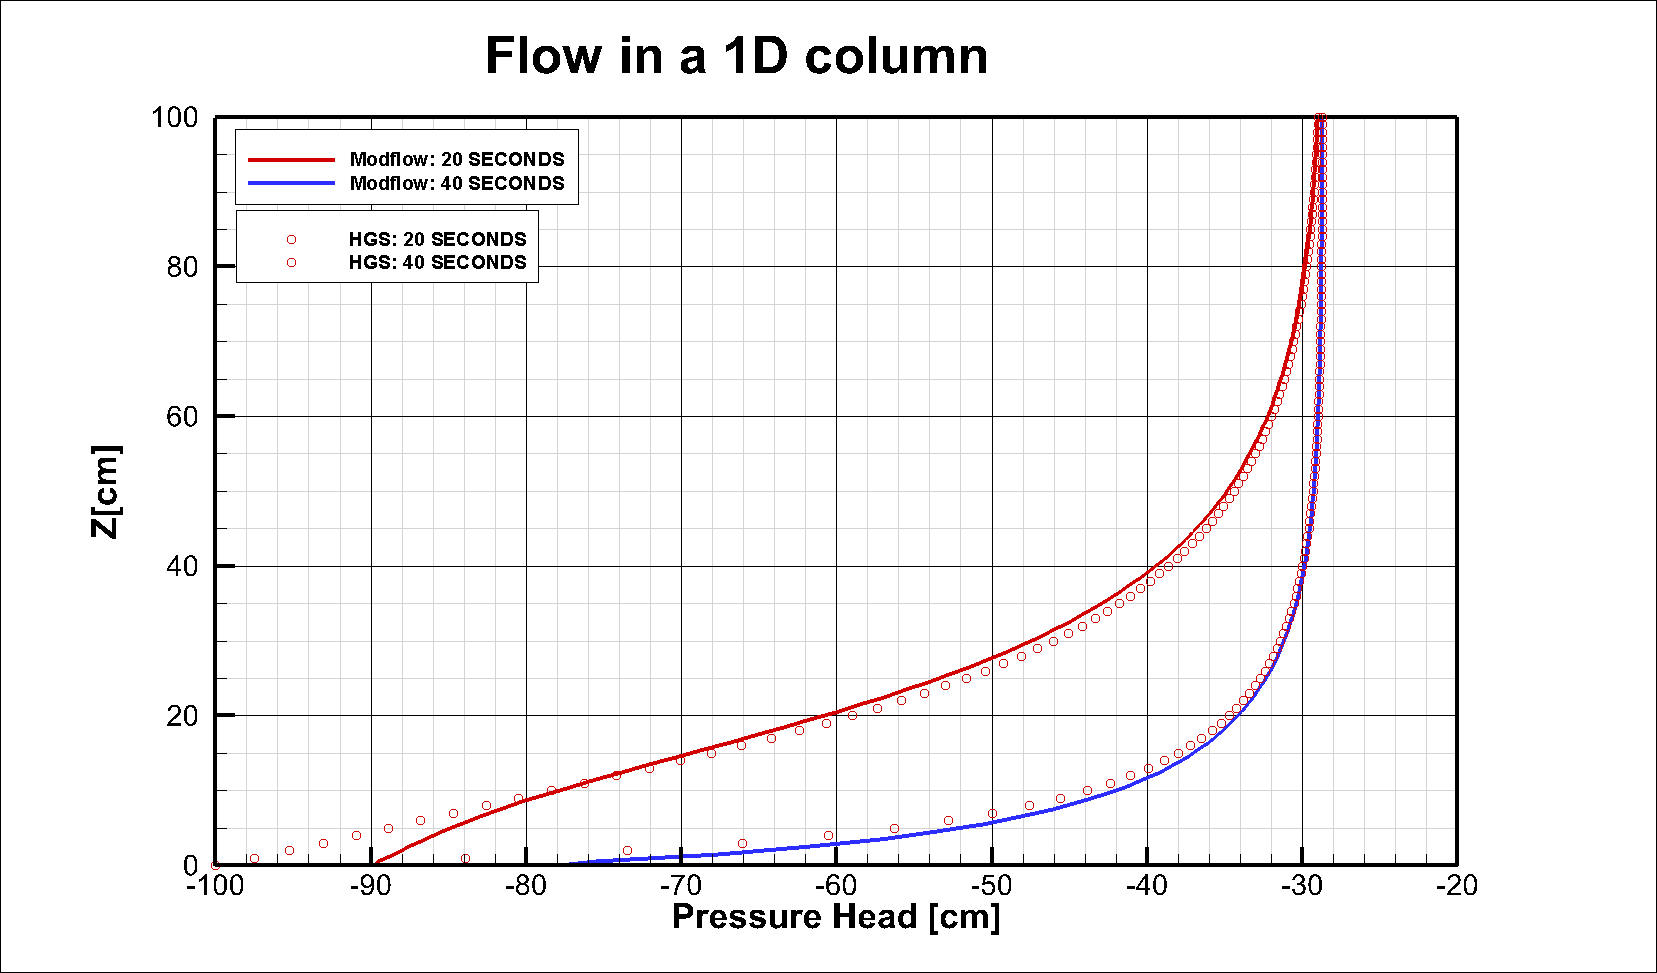
\includegraphics[width=0.87\textwidth]{1d_P_vs_Z}
    \vspace{.2in} \\

    Here is a comparison of saturation versus depth results for  \mfus\ and \hgs\ at 20 and 40 seconds:
    \vspace{.2in} \\
    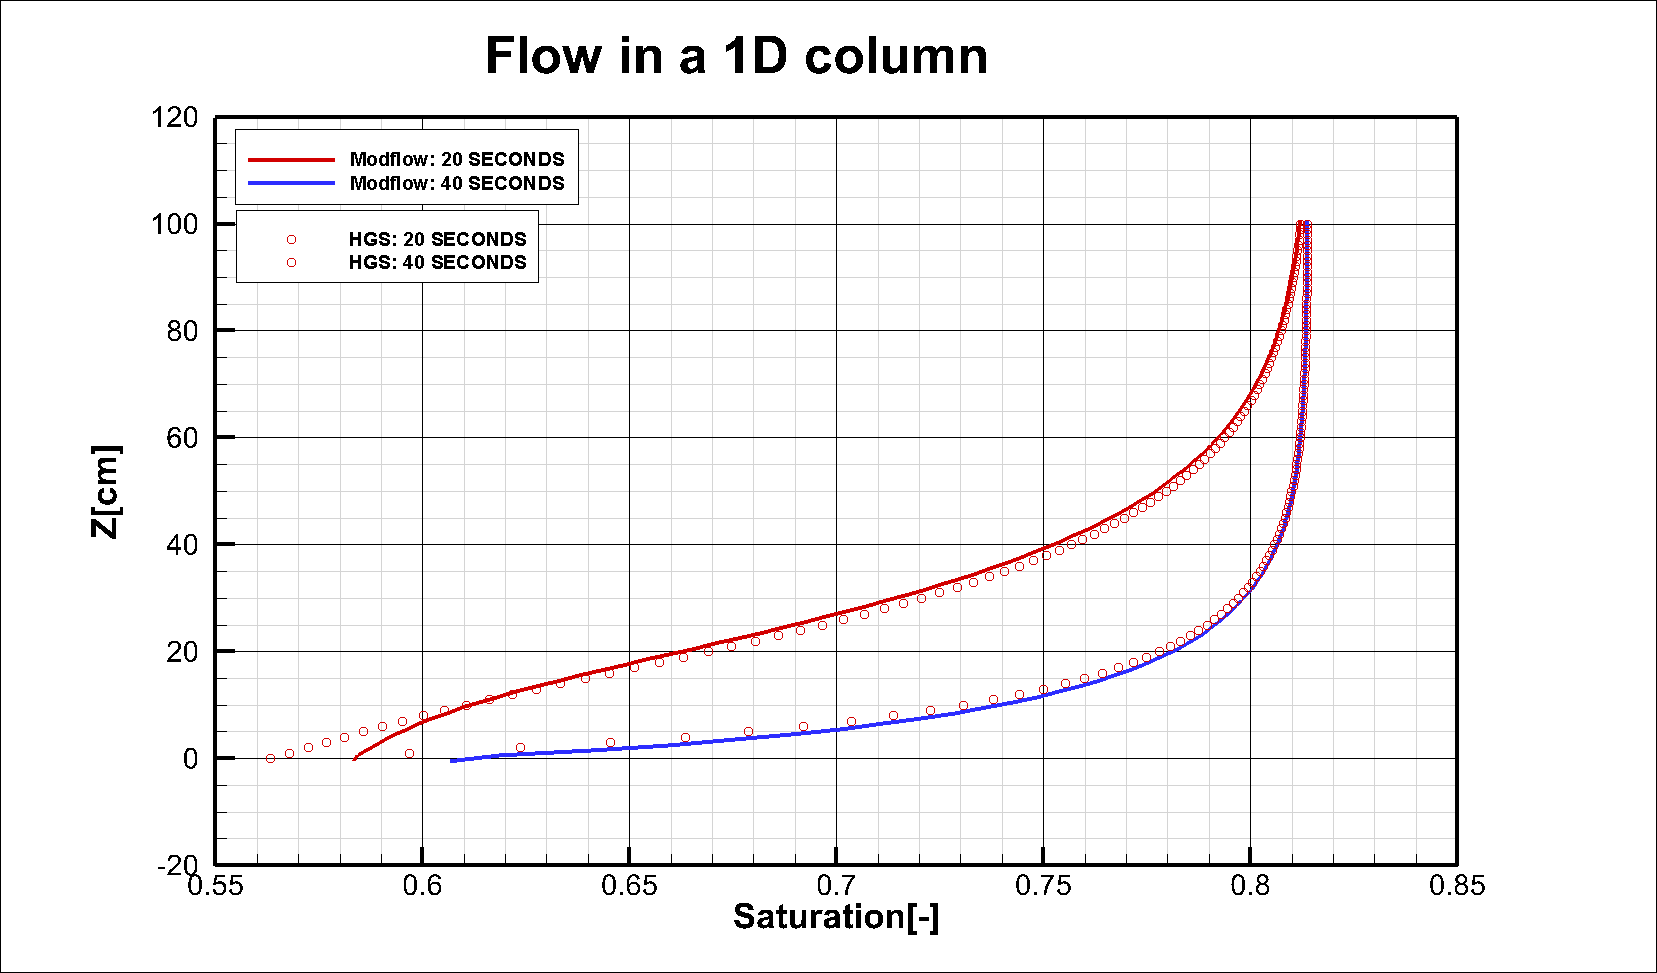
\includegraphics[width=0.87\textwidth]{1d_S_vs_Z}
    \vspace{.2in} \\

%
\includegraphics[width=.15\textwidth]{UnderConstruction} \textit{
%Although these results look good, there is a discrepancy between the unit systems used in the two models (e.g. K is 10 in \hgs\ and 1e-5 in \mfus.   HGS column height appears to be 100 cm, while \mfus\ model is 100 m thick.
%\mut\ needs to be modified to allow the user to change unit systems and then we should update this example.
%}




